\documentclass[11pt,a4paper]{article}

% ---------------------------------------------------------------- packages
\usepackage[T1]{fontenc}
\usepackage[utf8]{inputenc}
\usepackage{lmodern}
\usepackage[scaled=0.92]{helvet}
\usepackage{microtype}
\usepackage[margin=2.5cm]{geometry}
\usepackage{amsmath,amssymb}
\usepackage{graphicx}
\usepackage{booktabs,multirow,tabularx,array}
\usepackage{siunitx}
\usepackage[dvipsnames]{xcolor}
\usepackage{pifont}
\usepackage{tikz}
\usetikzlibrary{positioning,decorations.pathreplacing,calc}
\usepackage{algorithm}
\usepackage[noend]{algpseudocode}
\usepackage{caption}
\usepackage[section]{placeins}
\usepackage{enumitem}
\usepackage{titlesec}
\usepackage[style=numeric-comp,sorting=none,maxbibnames=4,giveninits=true,doi=true,url=false,isbn=false]{biblatex}
\addbibresource{references.bib}
\usepackage[hidelinks]{hyperref}
\usepackage[capitalise,noabbrev]{cleveref}

% Generated by scripts/make_figures.py -- do not edit by hand.
\newcommand{\alignSlope}{1.8}
\newcommand{\alignTimeMax}{0.5}
\newcommand{\arGEnd}{473}
\newcommand{\arGLen}{23}
\newcommand{\arGStart}{451}
\newcommand{\arQEnd}{80}
\newcommand{\arQLen}{23}
\newcommand{\arQStart}{58}
\newcommand{\arRawEnd}{473}
\newcommand{\arRawIdentity}{31}
\newcommand{\arRawLen}{430}
\newcommand{\arRawOffset}{1}
\newcommand{\arRawStart}{44}
\newcommand{\arRawZ}{66}
\newcommand{\colAlnIdentity}{55}
\newcommand{\colAlnScore}{87}
\newcommand{\colAlnZ}{7.4}
\newcommand{\colGlyFraction}{100.0}
\newcommand{\colPeakPeriod}{3.00}
\newcommand{\colPeakPower}{102}
\newcommand{\colRegionEnd}{1183}
\newcommand{\colRegionLen}{997}
\newcommand{\colRegionScore}{0.33}
\newcommand{\colRegionStart}{187}
\newcommand{\colSecondPower}{19}
\newcommand{\entropyTimeMax}{2}
\newcommand{\httAlnZ}{1.1}
\newcommand{\httLcrEnd}{85}
\newcommand{\httLcrStart}{11}
\newcommand{\httPEnd}{49}
\newcommand{\httPLen}{11}
\newcommand{\httPStart}{39}
\newcommand{\httQEnd}{38}
\newcommand{\httQLen}{21}
\newcommand{\httQStart}{18}
\newcommand{\nShuffles}{50}
\newcommand{\runtimeMaxLength}{4{,}000}
\newcommand{\supAlnA}{3--82}
\newcommand{\supAlnB}{21--101}
\newcommand{\supAlnIdentity}{52}
\newcommand{\supAlnOffset}{18}
\newcommand{\supAlnScore}{180}
\newcommand{\supAlnZ}{6.5}
\newcommand{\supUnit}{QQYNPQGGY}
\newcommand{\supUnitEnd}{90}
\newcommand{\supUnitStart}{71}
\newcommand{\tandemMinLength}{8}
\newcommand{\toyLength}{66}
\newcommand{\toyNyquistIndicator}{1.9}
\newcommand{\toyNyquistKD}{0.1}
\newcommand{\zSignificant}{4}


% ---------------------------------------------------------------- style
\definecolor{accent}{HTML}{2A78D6}
\definecolor{accent2}{HTML}{EB6834}
\definecolor{accent3}{HTML}{1BAF7A}
\definecolor{inkmuted}{HTML}{52514E}
\newcommand{\cmark}{\textcolor{accent3}{\ding{51}}}
\newcommand{\xmark}{\textcolor{inkmuted}{\ding{55}}}
\newcommand{\code}[1]{\texttt{#1}}
\newcommand{\seq}[1]{\texttt{#1}}

\captionsetup{font=small,labelfont={bf,sf},format=plain,margin=0.5em}
\titleformat{\section}{\large\bfseries\sffamily}{\thesection}{0.8em}{}
\titleformat{\subsection}{\normalsize\bfseries\sffamily}{\thesubsection}{0.8em}{}
\titleformat{\paragraph}[runin]{\normalsize\bfseries\sffamily}{}{}{}[.]
\setlist{itemsep=0.2em,topsep=0.4em}
\sisetup{group-separator={,},group-minimum-digits=4}
\hypersetup{pdftitle={Amino Acid Repeats: Analysis and Implications},pdfauthor={Ali Ahmadi Esfidi}}

\title{\sffamily\bfseries Amino Acid Repeats:\\[0.2em]\Large Analysis \& Implications}
\author{Ali Ahmadi Esfidi}
\date{Feb, 2025}

\begin{document}
\maketitle

% ================================================================ abstract
\begin{abstract}
\noindent Amino acid repeats (AARs) are abundant in protein sequences and play key roles in protein
function and evolution. Their variation is linked to disease: expansions of polyglutamine tracts
cause at least nine neurodegenerative disorders. This report reviews and implements four
complementary computational strategies for detecting AARs: sliding-window Shannon entropy
for low-complexity regions, a shifted self-match scan for tandem repeats, Fourier analysis
for periodic patterns, and Smith--Waterman self-alignment for diverged internal repeats.
A fifth method enumerates exact and BLOSUM-approximate repeated words.
We give a principled, normalised periodicity score with an exact interpretation through Parseval's theorem,
a vectorised self-alignment with Waterman--Eggert declumping and a shuffle-based significance estimate,
and an open, tested Python implementation. On a synthetic benchmark and four real proteins
(huntingtin, androgen receptor, collagen $\alpha$1(I) and yeast Sup35), each method recovers the
repeat class it is designed for and fails predictably on the others: entropy and tandem scanning
recover the disease-associated polyQ tracts exactly, only Fourier analysis
reveals the \num{\colRegionLen}-residue Gly-X-Y periodicity of collagen, and self-alignment
recovers the diverged oligopeptide repeats of Sup35 ($z=\supAlnZ$). We conclude that robust AAR annotation
requires combining methods, and that low-complexity masking is essential for alignment-based detection.
\end{abstract}

% ================================================================ introduction
\section{Introduction}\label{sec:intro}

Repetition is one of the most common architectural features of proteins. Surveys of sequence
databases estimate that a substantial fraction of proteins, and a larger fraction of eukaryotic
than prokaryotic proteins, contain internal repeats \cite{marcotte1999census}. AARs range from
runs of a single residue, such as the polyglutamine (polyQ) tract of huntingtin, through short
oligopeptide units, to entire structural domains of 20--40 residues that stack into solenoids
\cite{andrade2001repeats,kajava2012tandem}.

AARs matter for three reasons:
\begin{itemize}
  \item \textbf{Function and structure.} Repeated units build extended binding surfaces and fibres,
        as in the Gly-X-Y triple helix of collagen \cite{shoulders2009collagen}.
  \item \textbf{Evolution.} Repeats are mutational hotspots. Replication slippage and unequal crossing-over
        change copy number far faster than point mutation alters other sequence
        \cite{levinson1987slipped}, which makes repeats a source of rapid variation.
  \item \textbf{Disease.} Expansion of CAG codon repeats beyond a threshold produces expanded polyQ tracts and
        causes Huntington's disease, spinal and bulbar muscular atrophy and several spinocerebellar ataxias
        \cite{orr2007trinucleotide,hdcrg1993,laspada1991sbma}.
\end{itemize}

Because repeats are so heterogeneous, no single algorithm detects all of them. This report
(i) organises AARs into a classification framework (\cref{sec:classification}); (ii) describes and implements
four detection strategies with precise definitions (\cref{sec:methods}); (iii) evaluates them on a
synthetic sequence with known ground truth and on four well-characterised proteins (\cref{sec:results}); and
(iv) discusses their complementarity and the biological implications of repeats (\cref{sec:discussion}).

% ================================================================ classification
\section{Classification framework}\label{sec:classification}

We classify repeats along three independent axes (\cref{fig:classes}):
\begin{description}[leftmargin=1.2em,font=\sffamily\bfseries]
  \item[Unit similarity] \emph{Perfect} repeats have identical copies (\seq{MAMAMA}); \emph{imperfect}
        repeats tolerate substitutions or indels (\seq{PQGGYQQYN}/\seq{PQGGYQQQFN}).
  \item[Spatial arrangement] \emph{Tandem} copies are adjacent; \emph{distributed} (dispersed) copies are separated by
        unrelated sequence.
  \item[Pattern complexity] \emph{Simple} repeats have short units (1--10 residues) and low compositional
        complexity; \emph{domain} repeats have long units (typically 20--40 residues or more) that usually fold.
\end{description}
The axes matter because each detection strategy is sensitive to a different combination.
Low compositional complexity identifies simple repeats regardless of arrangement, periodicity
identifies tandem arrangements, and alignment identifies similarity regardless of arrangement.

\begin{figure}[tbp]
\centering
% Classes of amino acid repeats (shared by report and slides).
% Requires colours accent, accent2, accent3, inkmuted and xcolor's dvipsnames.
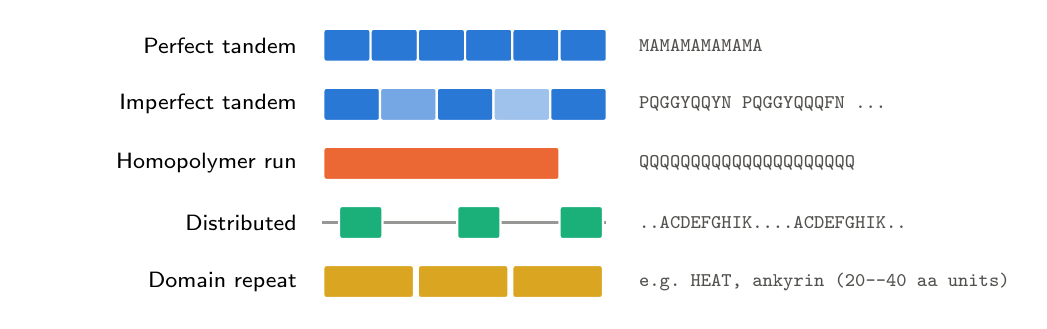
\begin{tikzpicture}[
  font=\sffamily\small,
  unit/.style={draw=white, line width=0.8pt, minimum height=0.42cm, inner sep=0pt, rounded corners=1pt},
  lab/.style={anchor=east, text width=3.3cm, align=right, font=\sffamily\footnotesize},
  note/.style={anchor=west, font=\ttfamily\scriptsize, text=inkmuted}]
  \def\row#1{-0.75*#1}
  % perfect tandem
  \node[lab] at (-0.2,{\row0}) {Perfect tandem};
  \foreach \i in {0,...,5} \node[unit, fill=accent, minimum width=0.6cm, anchor=west] at (0.6*\i,{\row0}) {};
  \node[note] at (3.9,{\row0}) {MAMAMAMAMAMA};
  % imperfect tandem
  \node[lab] at (-0.2,{\row1}) {Imperfect tandem};
  \foreach \i/\c in {0/accent,1/accent!65,2/accent,3/accent!45,4/accent} \node[unit, fill=\c, minimum width=0.72cm, anchor=west] at (0.72*\i,{\row1}) {};
  \node[note] at (3.9,{\row1}) {PQGGYQQYN PQGGYQQQFN \dots};
  % homopolymer
  \node[lab] at (-0.2,{\row2}) {Homopolymer run};
  \node[unit, fill=accent2, minimum width=3.0cm, anchor=west] at (0,{\row2}) {};
  \node[note] at (3.9,{\row2}) {QQQQQQQQQQQQQQQQQQQQQ};
  % dispersed
  \node[lab] at (-0.2,{\row3}) {Distributed};
  \draw[inkmuted!60, line width=1.2pt] (0,{\row3}) -- (3.6,{\row3});
  \foreach \x in {0.2,1.7,3.0} \node[unit, fill=accent3, minimum width=0.55cm, anchor=west] at (\x,{\row3}) {};
  \node[note] at (3.9,{\row3}) {..ACDEFGHIK....ACDEFGHIK..};
  % domain
  \node[lab] at (-0.2,{\row4}) {Domain repeat};
  \foreach \i in {0,1,2} \node[unit, fill=Goldenrod, minimum width=1.15cm, anchor=west] at (1.2*\i,{\row4}) {};
  \node[note] at (3.9,{\row4}) {e.g.\ HEAT, ankyrin (20--40 aa units)};
\end{tikzpicture}

\caption{Classes of amino acid repeats. Shading of the imperfect units indicates divergence from the consensus.
The three axes (unit similarity, spatial arrangement, pattern complexity) combine freely; a homopolymer run is
the limiting case of a perfect tandem repeat with a unit length of one.}
\label{fig:classes}
\end{figure}

% ================================================================ methods
\section{Methods}\label{sec:methods}

Throughout, $s = s_0 s_1 \cdots s_{n-1}$ is a protein sequence over the alphabet $\mathcal{A}$ of the
20 standard amino acids. Intervals are half-open and 0-based in the equations, and 1-based and inclusive
in tables and figures.

\subsection{Complexity: sliding-window Shannon entropy}\label{sec:entropy}
For a window $w = s_i \cdots s_{i+W-1}$ with residue frequencies $f_a$, the Shannon entropy \cite{shannon1948}
\begin{equation}
  H(w) = -\sum_{a\in\mathcal{A}} f_a \log_2 f_a \qquad (0 \le H \le \log_2 \min(W,20))
\end{equation}
measures compositional complexity. A homopolymer has $H=0$ and an alternating dipeptide has $H=1$.
All $n-W+1$ window entropies are computed in $O(n|\mathcal{A}|)$ time from cumulative one-hot counts.
Following SEG \cite{wootton1993seg}, a window with $H \le K_1$ (the \emph{trigger}) seeds a low-complexity
region (LCR). The region grows through contiguous windows with $H \le K_2$ (the \emph{extension}), and it is the
union of the residues of those windows. Because a window union overshoots the true boundary by up to $W-1$
residues, flanking residues that occur only once within the region are trimmed. We use SEG's standard
parameters $W=12$, $K_1=2.2$ and $K_2=2.5$ bits.

\subsection{Tandem repeats: shifted self-match}\label{sec:tandem}
For a period $p$, define the match indicator $m_i = [s_i = s_{i+p}]$. A run of $k$ consecutive ones means that
$s_i \cdots s_{i+k+p-1}$ is $p$-periodic, i.e.\ it contains $(k+p)/p$ copies of a $p$-residue unit. Scanning
$p = 1, \dots, 50$ costs $O(50\,n)$. Isolated substitutions break a run, so runs separated by short mismatch gaps
are bridged. A merge is accepted only if the appended run matches the current consensus unit in phase and the
merged region keeps a consensus identity of at least \SI{80}{\percent}. This rule prevents adjacent but
different homopolymers (such as \seq{Q$_{21}$P$_{11}$}) from being merged. Overlapping calls are resolved by
preferring longer regions and, for equal length, shorter periods, and every unit is reduced to its primitive
form (\seq{PPPP}$\to$\seq{P}, \seq{MAMA}$\to$\seq{MA}).

\subsection{Periodicity: Fourier analysis}\label{sec:fourier}
\paragraph{Encoding} Fourier methods need a numeric signal. A physico-chemical scale such as hydropathy
\cite{kyte1982hydropathy,hopp1981prediction,grantham1974difference,zimmerman1968characterization}
yields a single channel and underlies classic analyses such as the hydrophobic moment
\cite{eisenberg1984moment}. However, a scale collapses residues with similar values. On the
Kyte--Doolittle scale, M/A and S/T each differ by only 0.1, so \seq{(MA)$_n$} and \seq{(ST)$_n$} barely register.
We therefore default to the \emph{indicator} encoding, which has one binary channel per amino acid,
$x_{a,j} = [s_j = a]$ \cite{voss1992evolution}. On our synthetic sequence, the global relative power at period 2 is
\toyNyquistIndicator{} with the indicator encoding and only \toyNyquistKD{} with hydropathy.

\paragraph{Global spectrum} With $X_a(f) = \sum_j (x_{a,j}-\bar x_a)\,e^{-2\pi i f j}$, the relative power
\begin{equation}
  P(f) = \frac{\sum_a |X_a(f)|^2}{\sum_{a,j}(x_{a,j}-\bar x_a)^2}
\end{equation}
has mean $\approx 1$ over the non-zero Fourier frequencies $f = k/n$ (Parseval), so a peak value is directly an
enrichment factor over a featureless spectrum.

\paragraph{Local periodicity score} Global spectra dilute short repeats, so we score every window.
For a window of length $W_p$ (a multiple of $p$), let
\begin{equation}
  S_p = \frac{\sum_{a}\sum_{k=1}^{p-1} |X_a(k/p)|^2}{W_p \sum_{a}\sum_{j}(x_{a,j}-\bar x_a)^2}.
  \label{eq:sp}
\end{equation}
Because every harmonic $k/p$ is a Fourier frequency of the window, Parseval's theorem gives $0\le S_p\le 1$:
$S_p$ is \emph{the fraction of the window's variance explained by period-$p$ structure}. A perfectly
$p$-periodic window has $S_p = 1$, and a random window has $\mathbb{E}[S_p]\approx (p-1)/W_p$, since
$p-1$ of $W_p$ frequencies are counted. We report the baseline-corrected score
$E_p = (S_p - b_p)/(1-b_p)$ with $b_p = (p-1)/W_p$, clipped to $[0,1]$. All windows are evaluated in
$O(n|\mathcal{A}|p)$ time per period using prefix sums of $x_{a,j}e^{-2\pi i kj/p}$.
A $p$-periodic window is also periodic at every multiple of $p$, so the smallest period with
$E_p \ge \tau$ is taken as the primitive one.

\paragraph{Detection} Fourier analysis proposes, string matching verifies (\cref{alg:fourier}). Periods that
reach $E_p\ge\tau$ anywhere (plus their divisors) are passed to the tandem scanner of \cref{sec:tandem}, and
calls are kept only where the spectrum supports them. Some repeats are periodic \emph{in pattern} but do not
have identical units. Collagen's Gly-X-Y helix is the canonical example, because only every third residue is
conserved. For such cases we also report \emph{periodic regions}: maximal runs whose primitive period is
constant. Period~1 (homopolymer runs) cannot be seen by the DFT, because frequency 1 aliases to frequency 0;
the entropy and tandem methods cover it.

\begin{algorithm}[tbp]
\caption{Spectrum-guided tandem repeat detection}\label{alg:fourier}
\begin{algorithmic}[1]
\Require sequence $s$, periods $p_{\min}..p_{\max}$, window $W$, threshold $\tau$
\State $E \gets$ local excess scores $E_p(i)$ for all $p$, $i$ \Comment{\cref{eq:sp}, prefix sums}
\State $\hat p(i) \gets \min\{p : E_p(i) \ge \tau\}$ \Comment{primitive period at $i$}
\State $\mathcal{P} \gets \{d : d \mid \hat p(i)\text{ for some } i,\ d\ge p_{\min}\}$
\State $R \gets$ \Call{TandemScan}{$s$, $\mathcal{P}$} \Comment{shifted self-match, \cref{sec:tandem}}
\State \Return $\{r\in R : \max_{i\in r,\ q \,:\, r.p \mid q} E_q(i) \ge \tau\}$ \Comment{spectral support}
\end{algorithmic}
\end{algorithm}

\subsection{Self-comparison alignment}\label{sec:alignment}
Diverged repeats, both tandem and distributed, are found by aligning the sequence with itself
\cite{gibbs1970diagonal,heger2000radar,szklarczyk2004trust}. We fill the Smith--Waterman matrix
\cite{smith1981identification} with BLOSUM62 scores $\sigma$ \cite{henikoff1992blosum} and a linear gap
penalty $g=-8$:
\begin{equation}
  H_{i,j} = \max\{0,\ H_{i-1,j-1}+\sigma(s_i,s_j),\ H_{i-1,j}+g,\ H_{i,j-1}+g\},
\end{equation}
restricted to the upper triangle $j>i$ to exclude the trivial diagonal and its mirror image. Each row is computed in vectorised form:
with $E_j = \max\{0, H_{i-1,j-1}+\sigma, H_{i-1,j}+g\}$, the horizontal term is a running maximum,
$H_{i,j} = gj + \max_{k\le j}(E_k - gk)$, segmented at masked cells.

\paragraph{Declumping} The highest cell of the matrix spawns many overlapping ``shadow'' alignments, a problem
that dominated the output of the original prototype. Following Waterman and Eggert \cite{waterman1987eggert},
after each reported alignment its path cells are forced to zero and the matrix is recomputed from the first
affected row. Alignments whose two segments both overlap a previously reported pair by more than
\SI{50}{\percent} are skipped as register-shifted duplicates.

\paragraph{Low-complexity masking and significance} Compositionally biased regions produce high-scoring but
uninformative self-alignments (\cref{sec:res-alignment}), so LCRs found by \cref{sec:entropy} are optionally
replaced with \seq{X} before alignment, as is standard for BLAST and RADAR. Significance is estimated with a
$z$-score against the best self-alignment scores of \nShuffles{} shuffled sequences, permuting residues only
among unmasked positions. Because the null describes the \emph{best} alignment, $z$-scores of lower-ranked
alignments are conservative.

\subsection{Repeated words: exact and approximate}\label{sec:words}
The original prototype enumerated repeated substrings with a polynomial rolling hash \cite{karp1987rabin}
computed in 64-bit integers. For words longer than about eight residues the hash overflows, so unrelated words
were silently merged and repeats were missed. We replace it with an Apriori-style growth. A word of length $L$
can occur $k$ times only if its length-$(L-1)$ prefix does, so only surviving start positions are extended, and
the search stops at the longest repeated word. In approximate mode, every repeated word seeds a vectorised scan
that accepts windows whose BLOSUM62 score reaches a fraction $\theta=0.85$ of the word's self-score. Finally,
candidates are ranked by coverage (copies $\times$ length) and accepted greedily without overlap.

\subsection{Implementation and data}\label{sec:data}
All methods are implemented in the Python package \code{aarepeats}, which depends only on
NumPy \cite{harris2020numpy}, Matplotlib \cite{hunter2007matplotlib} and Biopython \cite{cock2009biopython}
(for substitution matrices). A unit-test suite of 21 tests covers known-answer cases for every
detector. One script (\code{scripts/make\_figures.py}) regenerates every figure, table and number in
this report. Sequences were taken from UniProtKB/Swiss-Prot \cite{uniprot2023} (\cref{tab:dataset}). Unless stated
otherwise, parameters are: entropy $W=12$, $K_1=2.2$, $K_2=2.5$; tandem minimum length \tandemMinLength{},
single-gap bridging, \SI{80}{\percent} identity; Fourier $W=12$, $\tau=0.5$ (verified repeats) and $W=36$,
$\tau=0.2$, minimum length 30 (periodic regions); alignment $g=-8$, minimum score 35, LCR masking on.

\begin{table}[tbp]
\centering
\caption{Proteins analysed. Each carries a well-documented repeat of a different class.}
\label{tab:dataset}
\small
\begin{tabular}{@{}lllll@{}}
\toprule
Protein & Gene & UniProtKB & Organism & Length \\
\midrule
Huntingtin & HTT & P42858 (v2) & \textit{H. sapiens} & 3{,}142 \\
Androgen receptor & AR & P10275 (v3) & \textit{H. sapiens} & 920 \\
Collagen $\alpha$1(I) chain & COL1A1 & P02452 (v6) & \textit{H. sapiens} & 1{,}464 \\
Eukaryotic release factor 3 (Sup35) & SUP35 & P05453 (v1) & \textit{S. cerevisiae} & 685 \\
\bottomrule
\end{tabular}

\end{table}

% ================================================================ results
\section{Results}\label{sec:results}

\subsection{Synthetic benchmark}\label{sec:res-toy}
The \toyLength-residue synthetic sequence used in the original notebooks contains three perfect tandem repeats,
three homopolymer runs and one non-repetitive spacer (\cref{tab:toy}, \cref{fig:toy}). Entropy and tandem
scanning recover every repeat element, and both correctly leave the spacer unflagged. Fourier analysis recovers all
three periodic repeats and, as expected, none of the homopolymers. Self-alignment recovers everything but also
flags the spacer. The spacer is caught in a long gapped alignment at a small diagonal offset that is anchored by
the flanking repeats. This is the false positive that motivates low-complexity masking. Exact word enumeration
misses (H)$_4$ and (W)$_5$ because they do not contain three non-overlapping copies of any word of length two or more.

\begin{table}[tbp]
\centering
\caption{Ground truth recovery on the synthetic sequence. \cmark: at least half of the element's residues are
covered by a call of that method. The spacer is a negative control, so a \cmark{} in that row is a false positive.
Toy parameters: entropy $W=8$, $K_1=1.5$, $K_2=2.0$; Fourier $W=8$; tandem minimum length 4; words with at least three copies.}
\label{tab:toy}
\small
\begin{tabular}{@{}lllccccc@{}}
\toprule
Element & Residues & Class & Entropy & Tandem & Fourier & Self-align. & Words \\
\midrule
(MA)$_6$ & 1--12 & perfect tandem & \cmark & \cmark & \cmark & \cmark & \cmark \\
(A)$_6$ & 26--31 & homopolymer & \cmark & \cmark & \xmark & \cmark & \cmark \\
(H)$_4$ & 32--35 & homopolymer & \cmark & \cmark & \xmark & \cmark & \xmark \\
(ST)$_{5}$S & 38--48 & perfect tandem & \cmark & \cmark & \cmark & \cmark & \cmark \\
(SG)$_{4}$S & 49--57 & perfect tandem & \cmark & \cmark & \cmark & \cmark & \cmark \\
(W)$_5$ & 58--62 & homopolymer & \cmark & \cmark & \xmark & \cmark & \xmark \\
PRTEINSEQENCE & 13--25 & non-repeat spacer & \xmark & \xmark & \xmark & \cmark & \xmark \\
\bottomrule
\end{tabular}

\end{table}

\begin{figure}[tbp]
\centering
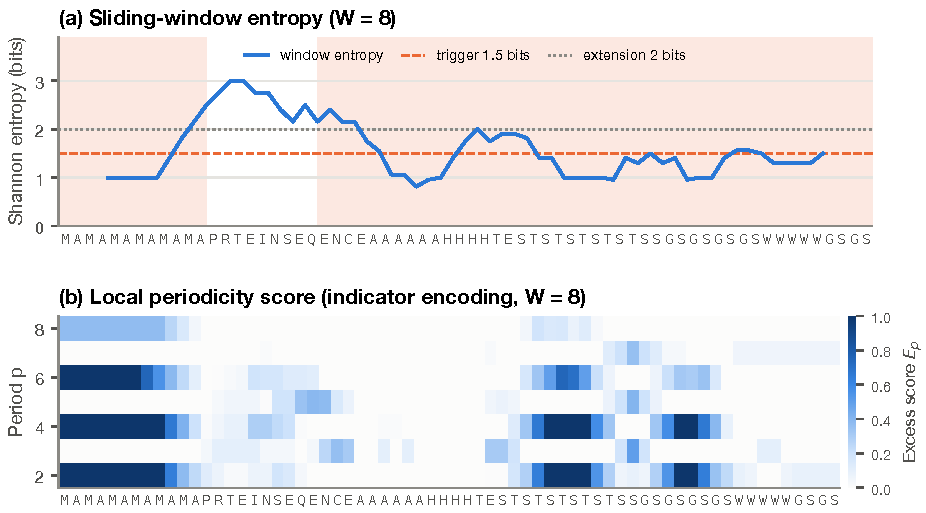
\includegraphics[width=\linewidth]{figures/toy.pdf}
\caption{Synthetic sequence. (a)~Window entropy with trigger and extension thresholds; shaded residues are the
detected LCRs. (b)~Local excess periodicity score $E_p$. The dipeptide repeats \seq{(MA)$_6$}, \seq{(ST)$_5$S} and
\seq{(SG)$_4$S} score $E_2=1$, with the expected echoes at the multiples $p=4,6,8$.}
\label{fig:toy}
\end{figure}

\subsection{Homopolymer tracts: huntingtin and the androgen receptor}\label{sec:res-polyq}
In huntingtin, the tandem scanner reports a perfect \seq{Q$_{\httQLen}$} tract at residues
\httQStart--\httQEnd, followed immediately by \seq{P$_{\httPLen}$} at \httPStart--\httPEnd. The two are kept
separate by the consensus-aware bridging rule. The entropy method reports a single
LCR (\httLcrStart--\httLcrEnd) that spans both tracts and the proline-rich region that follows
(\cref{fig:entropy}a). In the androgen receptor, the method reports \seq{Q$_{\arQLen}$} (\arQStart--\arQEnd)
and \seq{G$_{\arGLen}$} (\arGStart--\arGEnd), which appear as the two deepest entropy minima of the whole protein
(\cref{fig:entropy}b). These are the tracts whose expansion causes Huntington's disease and spinal and bulbar
muscular atrophy (\cref{sec:implications}). \Cref{tab:tandem} lists the longest tandem repeats in every protein.

\begin{figure}[tbp]
\centering
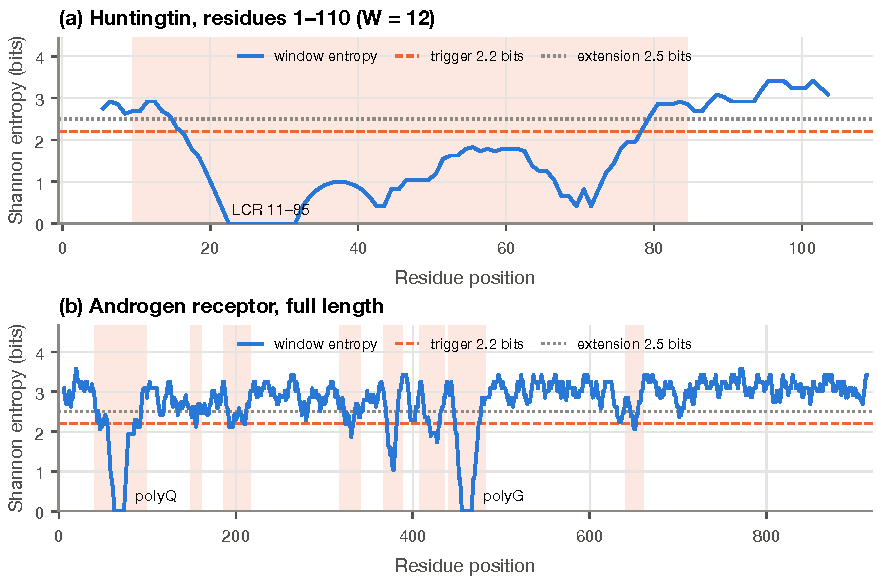
\includegraphics[width=\linewidth]{figures/entropy.pdf}
\caption{Sliding-window Shannon entropy ($W=12$). Shaded regions are LCRs detected with SEG's trigger and
extension thresholds. Homopolymer tracts drive the entropy to zero.}
\label{fig:entropy}
\end{figure}

\begin{table}[tbp]
\centering
\caption{Longest tandem repeats (up to five per protein) from the shifted self-match scan with single-gap bridging.
Identity is the fraction of residues matching the consensus unit.}
\label{tab:tandem}
\small
\begin{tabular}{@{}lrlrrr@{}}
\toprule
Protein & Residues & Unit & Period & Copies & Identity (\%) \\
\midrule
\multirow{4}{*}{HTT} & 18--38 & \texttt{Q} & 1 & 21.0 & 100 \\
 & 39--49 & \texttt{P} & 1 & 11.0 & 100 \\
 & 63--76 & \texttt{PQPQPPP} & 7 & 2.0 & 86 \\
 & 2649--2656 & \texttt{PSSP} & 4 & 2.0 & 88 \\
\addlinespace
\multirow{3}{*}{AR} & 58--80 & \texttt{Q} & 1 & 23.0 & 100 \\
 & 374--383 & \texttt{P} & 1 & 10.0 & 90 \\
 & 451--473 & \texttt{G} & 1 & 23.0 & 100 \\
\addlinespace
\multirow{5}{*}{COL1A1} & 138--154 & \texttt{PGP} & 3 & 5.7 & 94 \\
 & 326--344 & \texttt{GATGAAGPP} & 9 & 2.1 & 89 \\
 & 836--854 & \texttt{GDAGPPGPA} & 9 & 2.1 & 89 \\
 & 884--902 & \texttt{GPPGPSGNA} & 9 & 2.1 & 89 \\
 & 1175--1192 & \texttt{GPP} & 3 & 6.0 & 94 \\
\addlinespace
\multirow{4}{*}{SUP35} & 5--12 & \texttt{NQGN} & 4 & 2.0 & 88 \\
 & 71--90 & \texttt{QQYNPQGGY} & 9 & 2.2 & 100 \\
 & 179--188 & \texttt{TKEP} & 4 & 2.5 & 100 \\
 & 202--211 & \texttt{TEEK} & 4 & 2.5 & 90 \\
\bottomrule
\end{tabular}

\end{table}

\subsection{Periodic patterns: the collagen triple helix}\label{sec:res-collagen}
Collagen gives the clearest demonstration of what only spectral analysis can see. Its global spectrum has a
single dominant peak at period \colPeakPeriod{} with relative power \colPeakPower{}, more than five times the
next-highest frequency (\colSecondPower{}; \cref{fig:collagen}a). The local score localises it: a
period-3 region spans residues \colRegionStart--\colRegionEnd{} with mean $E_3=\colRegionScore$, and in that region
glycine occupies \SI{\colGlyFraction}{\percent} of the positions in one phase of the triplet (\cref{fig:collagen}b). The
score of about one third is itself informative. Only the glycine channel is perfectly periodic, while the X and Y
positions vary, so roughly a third of the indicator variance is periodic. Collagen therefore has no long identical
units: the tandem scanner fragments the helix into short pieces (\cref{tab:tandem}), and the entropy method marks
\SI{63}{\percent} of the protein as low-complexity without revealing why. Only the periodicity
analysis identifies the Gly-X-Y architecture.

\begin{figure}[tbp]
\centering
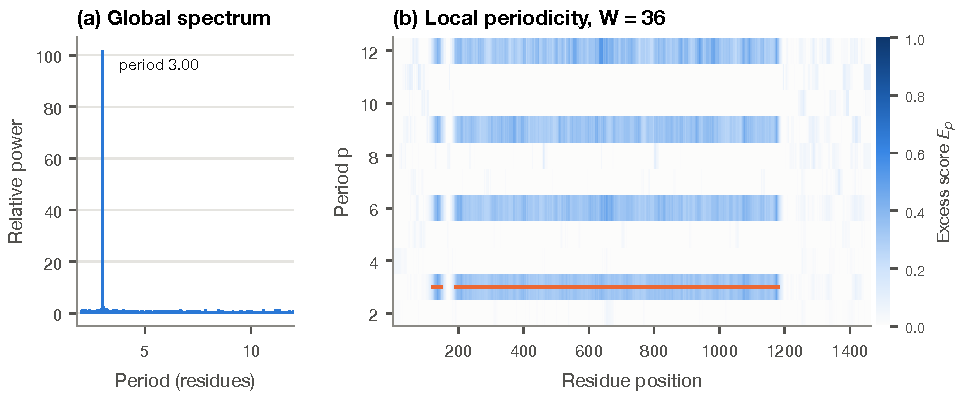
\includegraphics[width=\linewidth]{figures/fourier_collagen.pdf}
\caption{Collagen $\alpha$1(I). (a)~Global relative power spectrum (indicator encoding). (b)~Local excess
periodicity score; the orange line marks the detected period-3 regions. Bands at $p=6, 9, 12$ are the expected
echoes at multiples of the primitive period.}
\label{fig:collagen}
\end{figure}

\subsection{Diverged repeats: self-alignment}\label{sec:res-alignment}
The N-terminal domain of Sup35 contains imperfect oligopeptide repeats of the consensus
\seq{PQGGYQQYN} \cite{liu1999oligopeptide}. The tandem scanner finds only one exact two-copy stretch
(\seq{\supUnit}, residues \supUnitStart--\supUnitEnd), because the copies differ by substitutions and insertions.
Self-alignment of residues 1--125 instead recovers the whole repeat array as one alignment
(\supAlnA{} with \supAlnB; score \supAlnScore, identity \SI{\supAlnIdentity}{\percent}, $z=\supAlnZ$) at a diagonal
offset of \supAlnOffset{} residues, about two repeat units (\cref{fig:dotplot}a).

Low-complexity masking is not optional. Without masking, the best self-alignment of the androgen receptor
spans residues \arRawStart--\arRawEnd{} (\arRawLen{} residues, \SI{\arRawIdentity}{\percent} identity) at offset
\arRawOffset. In it, the polyQ, polyP and polyG tracts are chained through unrelated sequence into a single
``repeat'' with an apparent $z=\arRawZ$. With masking, no alignment reaches the score threshold. In collagen, masking
removes the dominant helix-wide alignment, and the surviving unmasked fragments still share significant Gly-X-Y
homology ($z=\colAlnZ$). For huntingtin, whose HEAT-like domain repeats are highly diverged, the best masked
alignment is not significant ($z=\httAlnZ$). Pairwise self-alignment with a general-purpose matrix is too
insensitive for such repeats, a limitation that profile- and structure-based methods address
(\cref{sec:discussion}). \Cref{fig:dotplot}b shows the masked analysis of a synthetic sequence, where the
dispersed copies of \seq{ACDEFGHIK} are recovered once the dominating dipeptide runs are masked.

\begin{figure}[tbp]
\centering
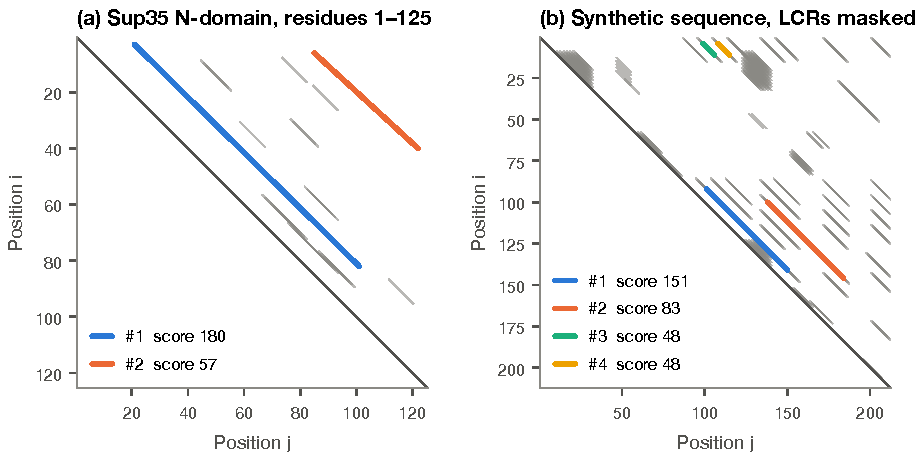
\includegraphics[width=\linewidth]{figures/dotplot.pdf}
\caption{Self-comparison. Grey strokes: filtered dot plot (at least 6 identities in a 9-residue diagonal window).
Coloured lines: non-redundant Smith--Waterman alignments after Waterman--Eggert declumping. (a)~Sup35 N-domain;
the main alignment links copies of the oligopeptide repeat two units apart. (b)~Synthetic sequence with LCRs masked.}
\label{fig:dotplot}
\end{figure}

\subsection{Whole-protein comparison}\label{sec:res-map}
\Cref{fig:map} and \cref{tab:summary} place all methods side by side. Their outputs overlap only partly.
Entropy flags compositionally simple regions, including some that are not repeats at all (for example,
hydrophobic stretches in huntingtin). The tandem scanner pinpoints exact units. Fourier analysis isolates
periodic architecture. Self-alignment, once masked, reports only relationships between complex segments.

\begin{figure}[tbp]
\centering
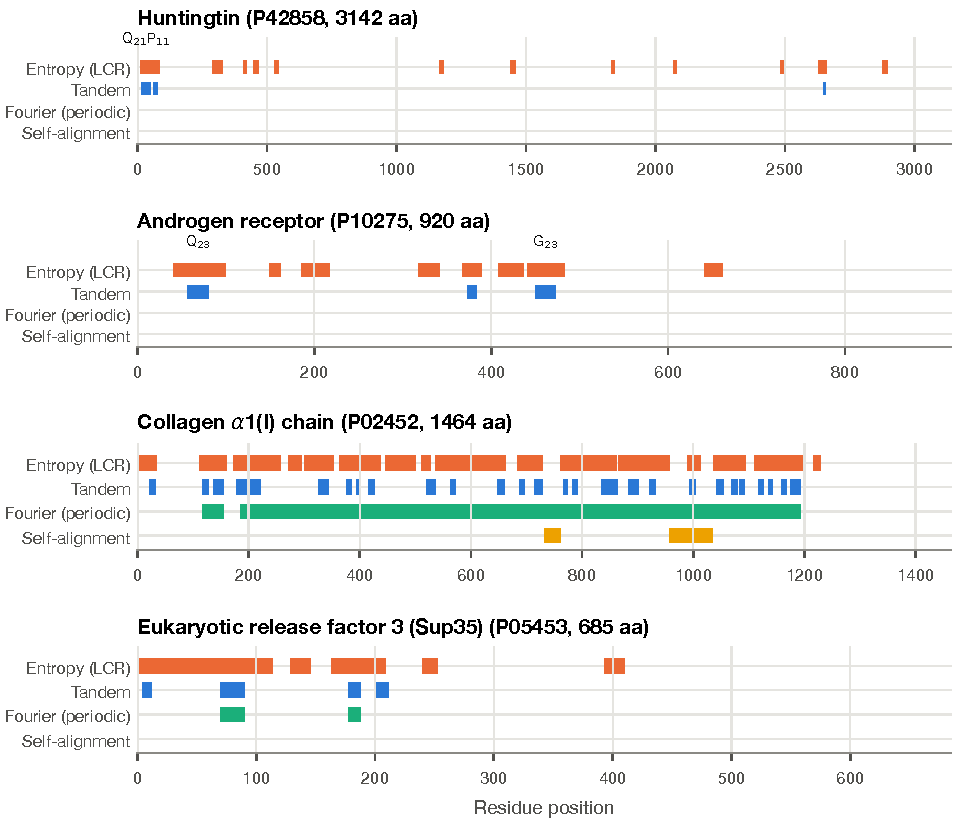
\includegraphics[width=\linewidth]{figures/repeat_map.pdf}
\caption{Repeat map of the four proteins. Each row shows the calls of one method; self-alignment shows segments of
masked alignments with $z\ge\zSignificant$.}
\label{fig:map}
\end{figure}

\begin{table}[tbp]
\centering
\caption{Summary per protein. Cover: percentage of residues in LCRs. Fourier verified: spectrally supported
tandem repeats. Self-alignment: best masked alignment and number with $z\ge\zSignificant$ (\nShuffles{} shuffles).}
\label{tab:summary}
\footnotesize
\setlength{\tabcolsep}{4pt}
\begin{tabular}{@{}lrrrrlrr@{}}
\toprule
 & \multicolumn{2}{c}{Entropy} & Tandem & \multicolumn{2}{c}{Fourier} & \multicolumn{2}{c}{Self-alignment (masked)} \\
\cmidrule(lr){2-3}\cmidrule(lr){4-4}\cmidrule(lr){5-6}\cmidrule(l){7-8}
Protein & LCRs & Cover (\%) & repeats & verified & periodic regions & top score ($z$) & $z \ge 4$ \\
\midrule
HTT & 13 & 8.8 & 4 & 0 & -- & 53 (1.1) & 0 \\
AR & 8 & 25.8 & 3 & 0 & -- & -- & 0 \\
COL1A1 & 19 & 63.3 & 30 & 14 & 119--151, 187--1183 ($p{=}3$) & 87 (7.4) & 2 \\
SUP35 & 5 & 30.1 & 4 & 2 & -- & -- & 0 \\
\bottomrule
\end{tabular}

\end{table}

\subsection{Computational cost}
\Cref{fig:runtime} shows wall time on random sequences of up to \runtimeMaxLength{} residues. Entropy and word
enumeration are effectively linear and take milliseconds. The tandem and Fourier scans scale linearly with a larger
constant, set by the number of periods. Self-alignment is quadratic in principle; the vectorised implementation
reaches an empirical exponent of \alignSlope{} and \SI{\alignTimeMax}{\second} at the largest size.
Every method is fast enough for proteome-scale screening of typical proteins.

\begin{figure}[tbp]
\centering
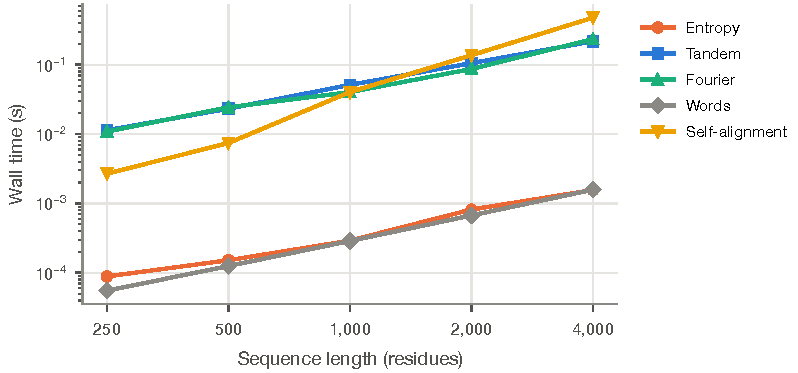
\includegraphics[width=0.66\linewidth]{figures/runtime.pdf}
\caption{Wall time against sequence length on random sequences (log--log; best of three runs up to 1,000 residues).
Self-alignment computes a single alignment.}
\label{fig:runtime}
\end{figure}

% ================================================================ discussion
\section{Discussion}\label{sec:discussion}

\subsection{Complementarity of detection strategies}
\Cref{tab:compare} summarises the strengths and blind spots that the results expose. In short, the class of a
repeat (\cref{sec:classification}) determines which method can find it, so a robust pipeline (i)~annotates LCRs
by entropy, (ii)~calls exact tandem units, (iii)~screens for periodic architecture spectrally, and (iv)~searches
for diverged relationships by self-alignment after masking the LCRs from step~(i).

\begin{table}[tbp]
\centering
\caption{Strengths and limitations of the detection strategies.}
\label{tab:compare}
\small
\begin{tabularx}{\linewidth}{@{}l>{\raggedright\arraybackslash}X>{\raggedright\arraybackslash}X@{}}
\toprule
Method & Detects well & Misses or misleads \\
\midrule
Entropy (SEG-style) & Homopolymers, short simple repeats, compositional bias; linear time
  & Diverged and domain repeats; flags non-repetitive biased regions; boundaries are only approximate \\
Tandem self-match & Exact or near-exact tandem units, with the unit and copy number
  & Distributed repeats; patterns with variable positions (Gly-X-Y); indels \\
Fourier & Periodic architecture without identical units; robust to substitutions
  & Homopolymers (period 1); non-periodic and distributed repeats; short repeats need short windows \\
Self-alignment & Diverged tandem and distributed repeats, with indels and significance estimates
  & Very diverged domain repeats; dominated by LCRs unless masked; quadratic cost \\
Repeated words & Exact or BLOSUM-similar dispersed motifs
  & Indels; spurious short words in long sequences \\
\bottomrule
\end{tabularx}
\end{table}

\paragraph{Machine learning implementations} Statistical methods such as these remain the backbone of repeat
annotation, but learned approaches are increasingly complementary. Profile-based iterative tools
such as RADAR \cite{heger2000radar} and TRUST \cite{szklarczyk2004trust} already improve on pairwise alignment for
diverged domain repeats. Accurate structure prediction \cite{jumper2021alphafold} makes it possible to detect
repeats as recurring structural units even when their sequences have diverged beyond recognition, and
classifiers trained on features such as the entropy, periodicity and alignment scores computed here are a
natural next step.

\subsection{Functional implications}\label{sec:implications}
\paragraph{Protein folding} Domain repeats fold into elongated solenoids (e.g.\ HEAT, ankyrin and leucine-rich
repeats) that present large surfaces for protein--protein interaction \cite{kajava2012tandem,andrade2001repeats}.
At the other extreme, the strict glycine periodicity found in collagen is a structural requirement: glycine
is the only residue small enough to occupy the centre of the triple helix \cite{shoulders2009collagen}.

\paragraph{Evolutionary conservation patterns} Repeat copy number is unstable because slipped-strand mispairing
and unequal crossing-over add or remove whole units \cite{levinson1987slipped}. Repeats therefore evolve faster
than their flanks, and variation in their length can tune function. In Sup35, changing the number of
oligopeptide repeats alters prion propagation \cite{liu1999oligopeptide}.

\paragraph{Neurological disease associations} Expansion of polyQ tracts underlies a family of dominantly inherited
neurodegenerative diseases \cite{orr2007trinucleotide}. In Huntington's disease, CAG repeats of 40 or more in
\emph{HTT} are fully penetrant, and 36--39 repeats show reduced penetrance \cite{hdcrg1993}. Expansion of the
androgen receptor CAG tract causes spinal and bulbar muscular atrophy \cite{laspada1991sbma}. Because the tract
length is visible directly in sequence, the detectors here can quantify it immediately (\cref{sec:res-polyq}).

\paragraph{Potential therapeutic targets} The direct link between repeat length and pathogenesis makes the
expanded gene product a therapeutic target. Antisense oligonucleotides that lower huntingtin expression have
been tested in patients \cite{tabrizi2019targeting}, and repeat-containing proteins in general are candidates for
strategies that reduce their expression or aggregation.

\subsection{Limitations}
Thresholds are heuristic: the SEG parameters are conventional rather than optimised, and the
Fourier threshold trades sensitivity against false periods. The shuffle $z$-score assumes an approximately normal
null for the maximum alignment score, whereas the true null is closer to an extreme-value distribution, so very
small $p$-values should not be read literally. Finally, the evaluation uses one synthetic sequence and four proteins
with well-known repeats; it illustrates the behaviour of each method but is not a benchmark of accuracy.

% ================================================================ conclusion
\section{Conclusion}
AARs are diverse, and so must be the methods that find them. Complexity measures, shifted self-matching,
Fourier analysis and self-alignment each reveal a different facet of repetition: homopolymer tracts, exact
tandem units, periodic architecture and diverged copies. On real proteins they recover the disease-associated
polyQ tracts of huntingtin and the androgen receptor, the Gly-X-Y periodicity of collagen, and the diverged
oligopeptide repeats of Sup35. Each method's failures are predictable from the repeat class. Combining the
methods, with low-complexity masking before alignment, gives a reliable picture of a protein's repetitive
architecture and of the regions where repeat variation is likely to have functional and clinical consequences.

\appendix
\section{Corrections to the original prototype}\label{app:changes}
The analysis rests on a re-implementation of the original notebooks and script. These defects were fixed:
\begin{enumerate}
  \item \textbf{Hash overflow.} The rolling hash in \code{repeat detector.py} was computed in \code{int64} with base 256,
        which overflows for words longer than about eight residues, so unrelated words collided. It was replaced
        by exact Apriori-style word growth (\cref{sec:words}).
  \item \textbf{Mislabelled scale.} The scale labelled ``Zimmerman polarity'' contained Grantham's polarity values
        \cite{grantham1974difference}. It is now labelled correctly.
  \item \textbf{No mean removal.} The Fourier analysis did not subtract the signal mean, used a single global
        spectrum and a single physico-chemical scale. It now uses mean-centred indicator channels and the normalised
        local score of \cref{eq:sp}.
  \item \textbf{Redundant alignments.} Self-alignment reported every cell above threshold, producing dozens of
        overlapping copies of the same repeat, and filled both triangles of the matrix. It now uses the upper triangle,
        Waterman--Eggert declumping, LCR masking and shuffle $z$-scores.
  \item \textbf{LCR boundaries.} Boundaries were derived from window centres with an asymmetric correction. Regions are now
        unions of qualifying windows with singleton trimming, using SEG's two thresholds.
  \item \textbf{Hygiene.} The deprecated Matplotlib style \code{seaborn-darkgrid}, unused code, a side-effecting
        cache file and file names containing spaces were removed. The code was packaged, tested and documented.
\end{enumerate}

\printbibliography[heading=bibintoc]

\end{document}
